\chapter{Nigoki: Schedule Replication System} \label{chap:schedrep}
In chapter ~\ref{chap:detexec} we described using a deterministic system to ensure the applications on the primary and secondary replica can have the same thread interleaving. The major advantage of the deterministic system is that we can minimize the communication between the replicas. However the downside is that we need to precisely adjust the logical time to maintain decent parallelism for multithreaded applications. We showed various solutions to balance the logical time because we need to keep the execution to be fast and deterministic. If all the burdens come from being deterministic, can we break the determinism once for all but still keep the replicas to be synchronized? The answer is yes.

In this chapter we are going to describe Schedule Replication for replicated applications. In this algorithm, we break the determinism entirely and use messages to synchronize every single synchronization primitives between the primary and replica. For an application that has massive number of synchronization primitives, this approach might introduce overheads from the communication, Figure~\ref{f:tradeoff} shows the relation between two different algorithms. Fortunately, our system is for inter-kernel replication, and Popcorn Linux provides a messaging layer with negatable latency. As a result having massive massages between replicas won't put too much overhead to the replication.

% !!!!!!!!!put this into conclusion
\begin{figure}
\centering
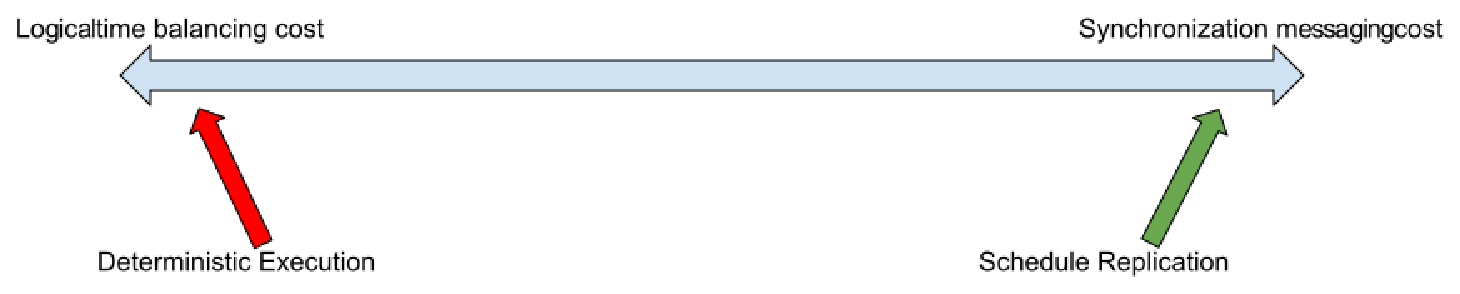
\includegraphics[width=0.8\columnwidth]{figures/tradeoff}
\caption{Trade off between two algorithms}
\label{f:tradeoff}
\end{figure}

% Discuss the latency benefit

\section{Execute-Log-Replay}
Before we get into the detail of this algorithm, let's revisit some important properties that are provided by the deterministic system.

\begin{itemize}
\item Serialization of deterministic areas. (The code region between detstart and detend).
\item Same total order of getting into deterministic areas on primary and secondary.
\end{itemize}

The first property is guaranteed by the fact that the logical time won't change during the execution of a deterministic area, and the second property is guaranteed by increasing the logical time in a same way on both primary and replica. As long as these two properties are guaranteed, the thread interleaving on both primary and secondary are sure to be the same (also for tick bump). In our Schedule Replication mode, we guarantee these two properties with the following approaches:

\begin{itemize}
\item Serialize deterministic areas with a global mutex on both primary and secondary.
\item Log the sequence of getting into deterministic areas on the primary and replay it on the secondary.
\end{itemize}

\begin{figure}
\begin{lstlisting}[numbers=left, frame=single, basicstyle=\small, breaklines]{schedrep}
void __det_start()
{
    if (is_secondary(current))
        wait_for_sync(current->seq, 
            ns->seq, current->ft_pid);
    lock(ns->global_mutex);
    current->ft_det_state = FT_DET_ACTIVE;
}
void __det_end()
{
    if (is_primary(current))
        send_sync(current->seq, 
            ns->seq, current->ft_pid);
    current->seq++;
    ns->seq++;
    current->ft_det_state = FT_DET_INACTIVE;
    unlock(ns->global_mutex);
}
\end{lstlisting}
\caption{Simplified implementation of system calls for schedule replication}
\label{f:schedrep_c}
\end{figure}

% explain something for tha variables
% reference to ft_pid
% why I dont need to handle I/O

Here we still use \detstart\ and \detend\ to wrap around a code section that needs to be synchronized with the replica. Figure~\ref{f:schedrep_c} shows a simplified version of \detstart\ and \detend\ in Schedule Replication.  Every thread in the namespace maintains a sequence number $Seq_{thread}$ and the entire namespace maintains a sequence number $Seq_{global}$. On the primary, \detstart\ simply locks the global mutex, \detend\ unlocks the global mutex, sends a tuple of $< Seq_{thread}, Seq_{global}, ft\_pid >$ to the secondary and then increase the value of $Seq_{global}$ and $Seq_{thread}$. On the secondary, \detstart\ blocks until it receives a $< Seq_{thread}, Seq_{global}, ft\_pid >$ tuple corresponds to its caller thread, then holds the global mutex, and \detend\ increases $Seq_{global}$ and $Seq_{thread}$, then release the global mutex.


Figure~\ref{f:scherep} shows an example of how Schedule Replication works in action.

\begin{figure}
\centering
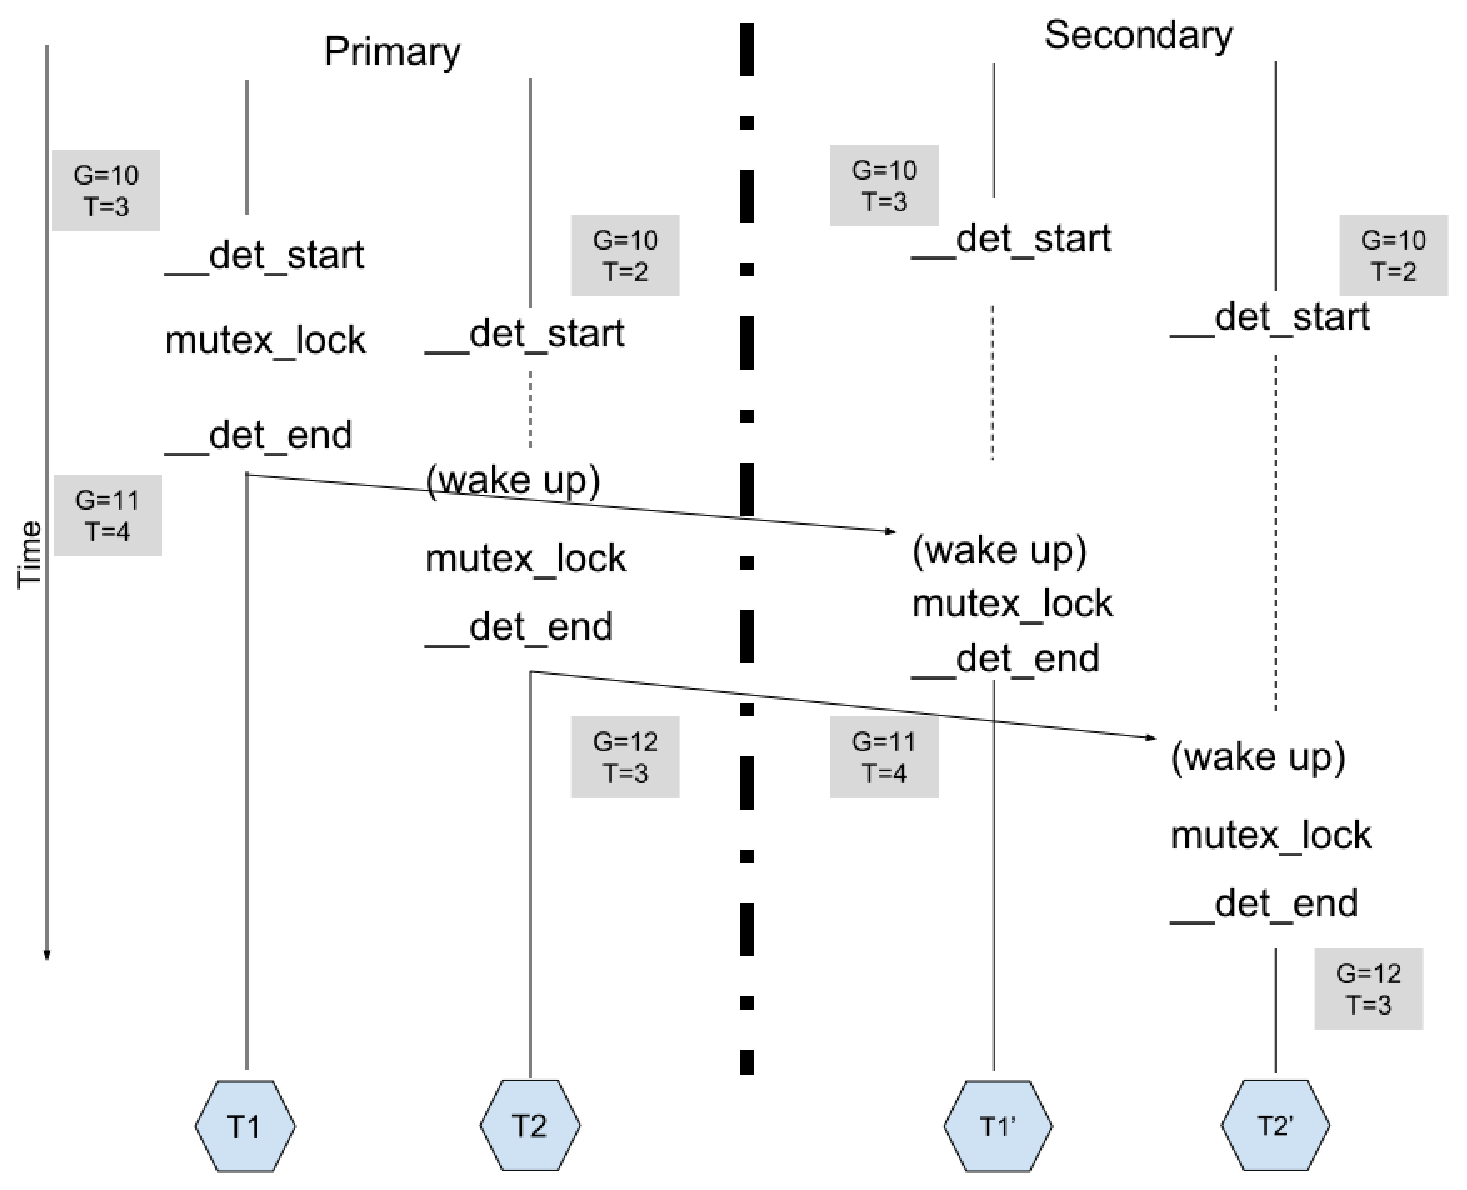
\includegraphics[width=0.9\columnwidth]{figures/sched_rep}
\caption{An example of Schedule Replication}
\label{f:scherep}
\end{figure}

\section{Related Work}

%doublePlay

%REX
Partial order

%ALL about EVE
